% !TEX encoding = UTF-8
% !TEX TS-program = pdflatex
% !TEX root = ../Tesi.tex
% !TEX spellcheck = en-EN

%************************************************
\chapter{Artificial Neural Network}
\label{cap:ann}
%************************************************

\section{Regression statistic}
\label{sec:regressionstatistic}

We start with a set of random variables, aiming to find a relationship between
them. We choose one of them ($response$), and we infer its dependance from the
others ($regressors$), also including an additive $error$ term. We call this a
\textit{regression model}, which can be linear or nonlinear.
The Bayesian linear and the Gaussian non linear regressions 
can be used as regression methods for \acs{DEM} identification
and to further
assess the quality of the \acs{ANNs} training.

\section{ANN intro}
\label{sec:annintro}
%\improvement{Add some more details from Haykin introduction}
An Artificial Neural Network (\acs{ANN}) is a powerful regression model, 
based on non-linear functions (Haykin \cite{RefWorks:158}). 
In fact, we can see a neural network as a huge and parallel computer, composed
of many processing units. It stores experienced knowledge and translates it in
an usable form. 
The biological inspiration for artificial neural networks can be seen in Fig.
\ref{fig:049neuron1}. It resembles the human brain especially because it
uses a learning process to acquire knowledge, which is stored through the
synaptic weights.

\begin{figure}[!htb]
\centering
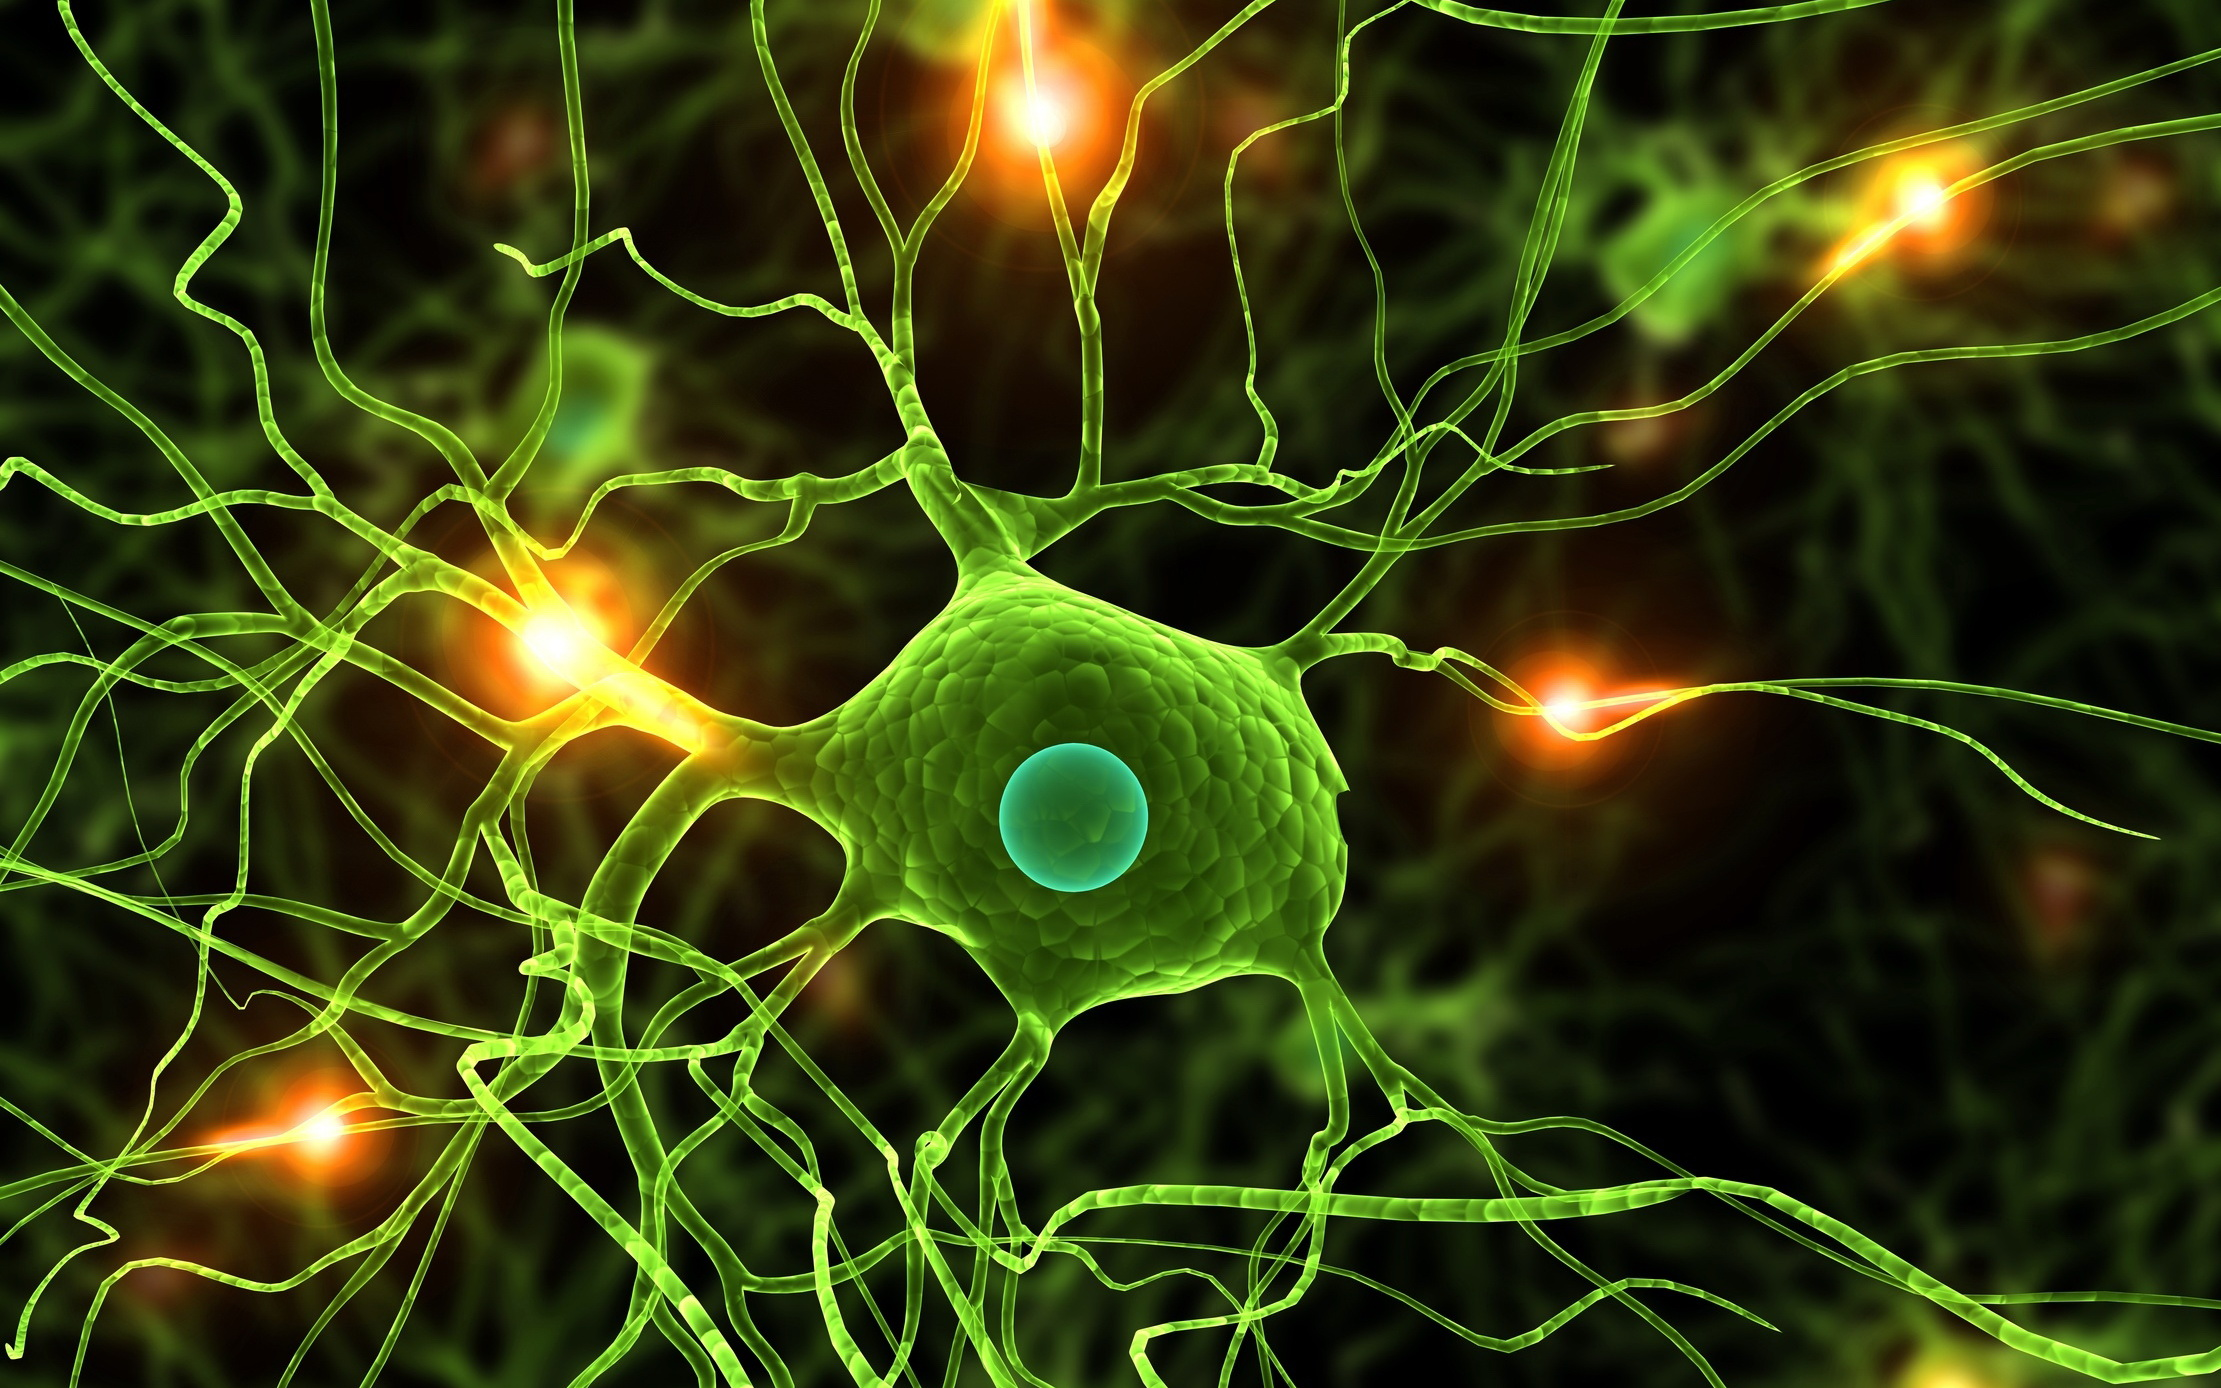
\includegraphics[width=.80\columnwidth]{images/049neuron1}
\caption[Biological inspiration 2]{Biological inspiration 2.}
\label{fig:049neuron1}
\end{figure}

In this work, we first used the \acs{ANN} to fit the \acs{DEM} numerical simulation
data, and then to process a vast number of parameters combinations. 
\acs{ANNs} map combinations of input data to convenient outputs (fitting). 
There is a variety of \acs{ANNs} available; important for our context were the
Feedforward (\acs{FF}) and the Radial basis function (\acs{RBF}). 
For \acs{FF}-\acs{ANN},
numerous training algorithms are available. The most common are based on
backpropagation, e.g., Levenberg-Marquardt, Bayesian regulation and the scaled
conjugate gradient.

\section{Perceptron}
\label{sec:perceptron}

The basic element of an artificial neural network is the perceptron, see Fig.
\ref{fig:064perceptron}, that is mathematically described by equation
\ref{eq:perceptron}: 
\begin{equation}
y = \varphi(b + \sum_{j = 1}^{m}{w_j \cdot x_j}),
 \label{eq:perceptron}
\end{equation}

where $x_j$ are the input nodes, $y$ is the output node, $w_j$ are the weights
and $b$ is the bias.
\begin{figure}[!htb]
\centering
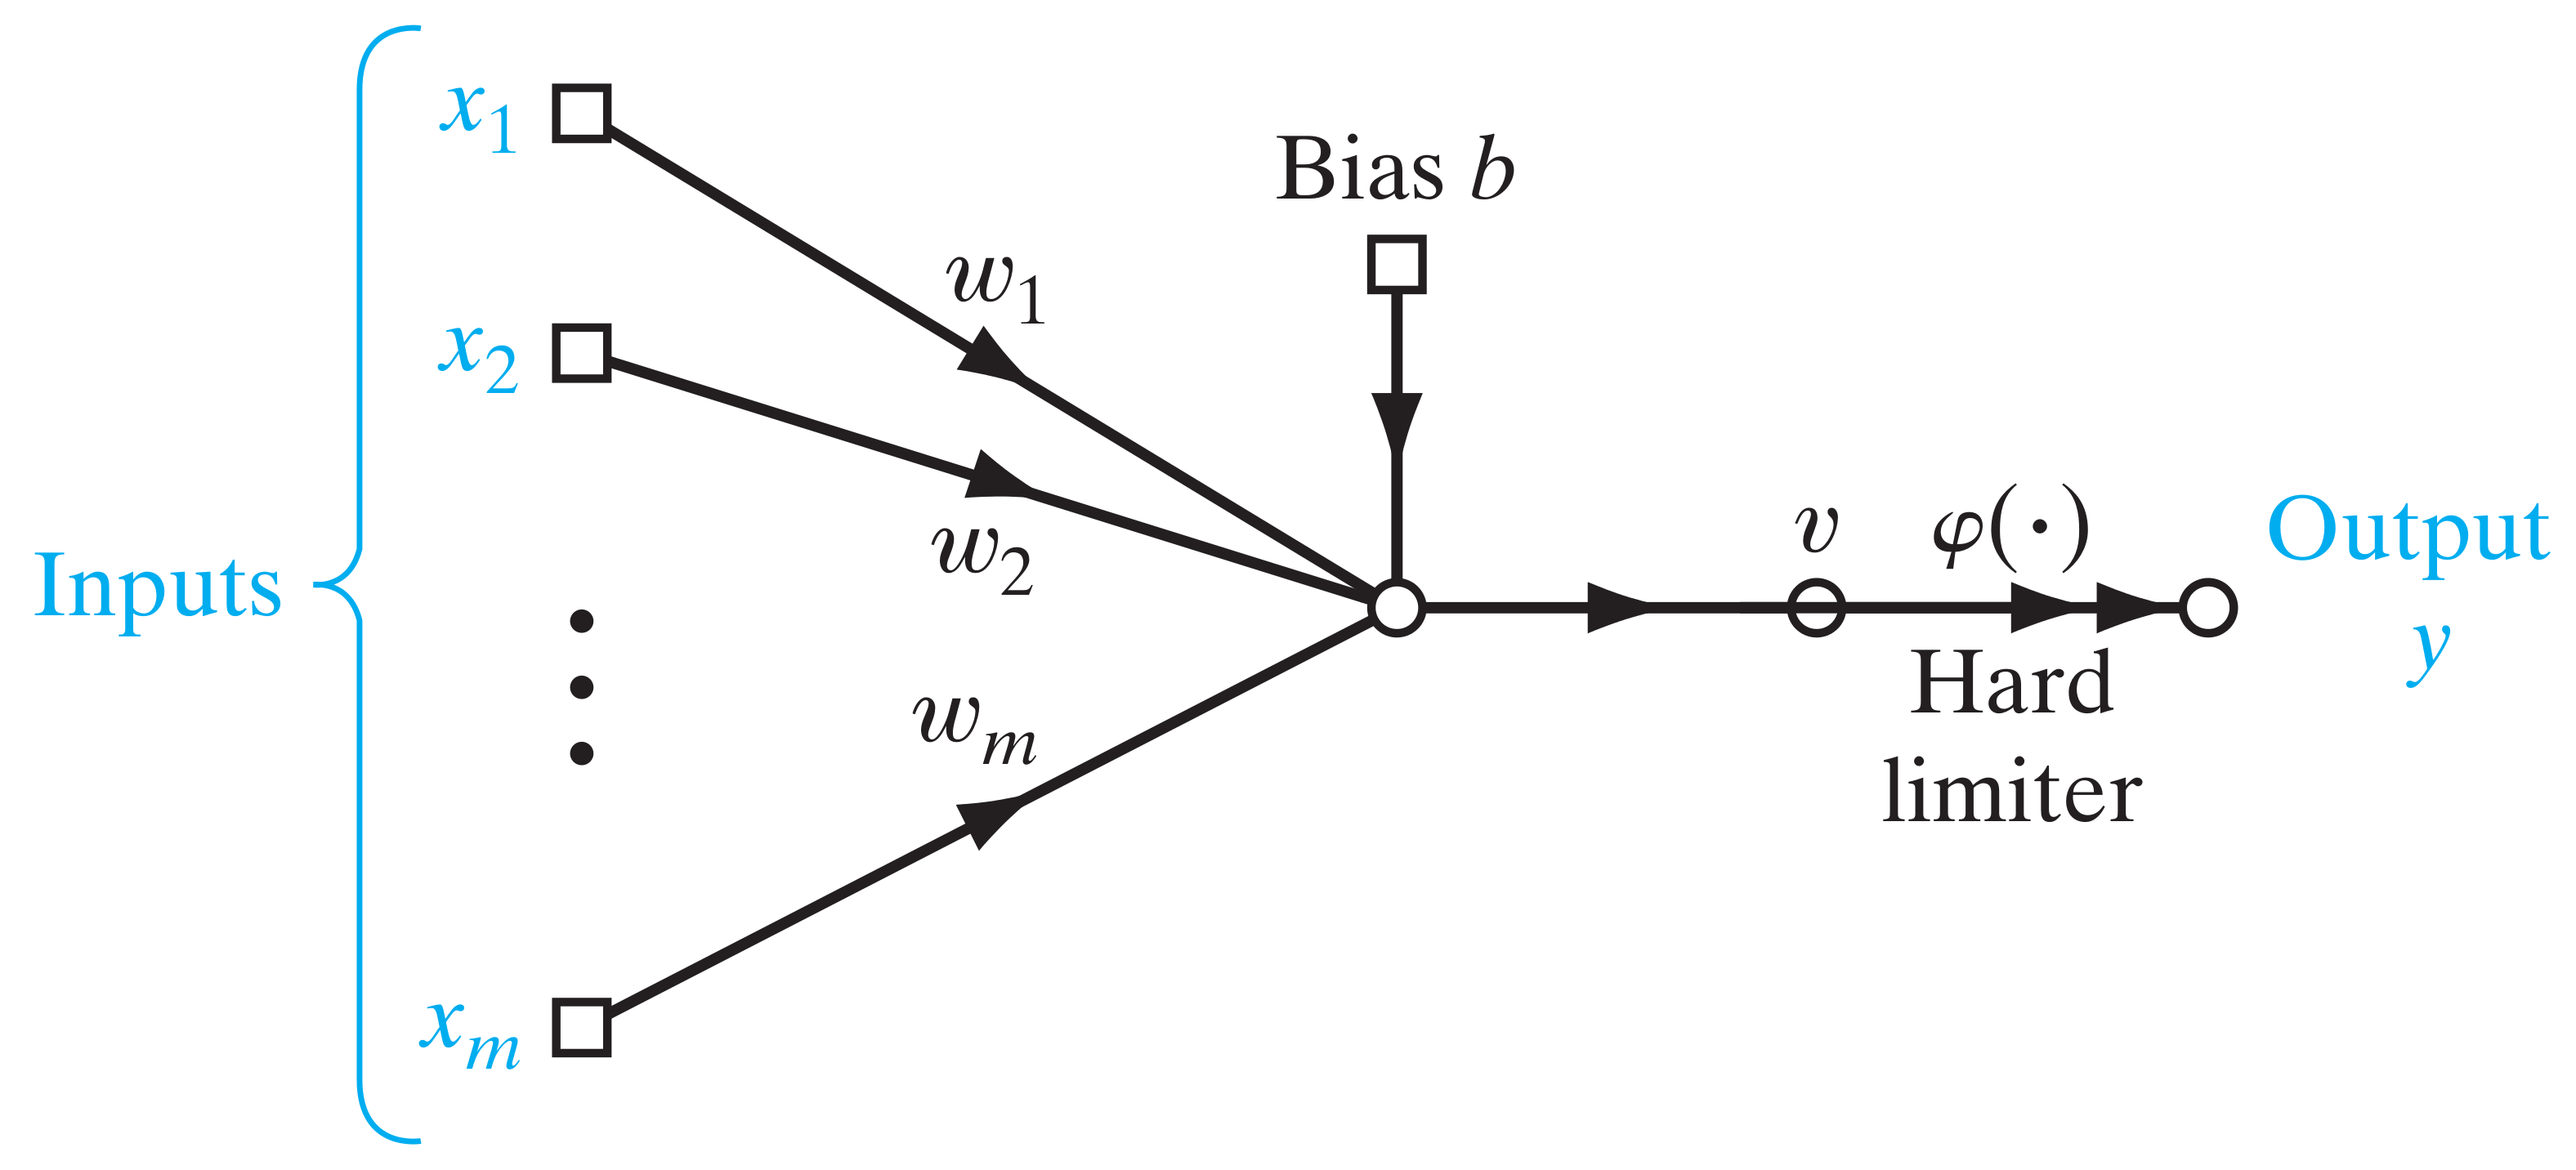
\includegraphics[width=.80\columnwidth]{images/064perceptron}
\caption[Perceptron scheme]{Perceptron scheme \cite{RefWorks:158}.}
\label{fig:064perceptron}
\end{figure}
In the simplest case  the activation function $\varphi(\cdot)$ is an hard
limiter, or a signum function.
Consequently, $y$ can be +1, for positive inputs, or -1, for negative inputs. Inputs of the first class
belong to class $\mathscr{C}_1$, of the second to class $\mathscr{C}_2$.
Thus, the patterns ($y$) are hypothesised to be linearly separable.
In this case the training, as identification of the correct weights and bias,
can be precisely mathematically described.
\begin{figure}[!h]
\centering
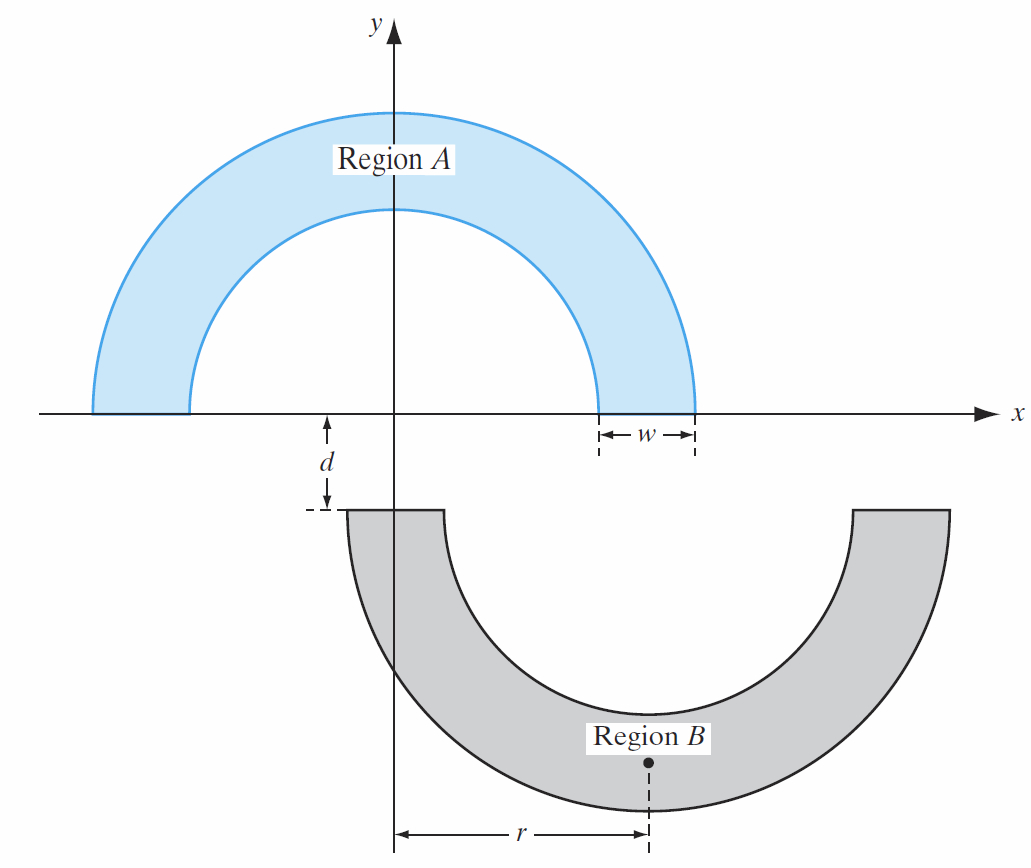
\includegraphics[width=.6\columnwidth]{images/105doublemoon2}
\caption[Double moon scheme]{Double moon scheme \cite{RefWorks:158}.}
\label{fig:105doublemoon2}
\end{figure}
The classical example of the double moon, see Fig. \ref{fig:105doublemoon2},
which clarifies the limits of the single perceptron approach, especially 
why a single neuron is not capable to handle a
nonlinear problem.
As long as the distance $d$ is positive, the domain can easily be
linearly separated in two regions.

%\improvement{better and more detailed explanation about the double moon}
%\improvement{Add some more details about the perceptron from Haykin}
\section{Multilayer}
\label{sec:multilayer}

\begin{figure}[!h]
\centering
\includegraphics[width=.70\columnwidth]{images/063doublemoon}
\caption[Double moon classification problem 1]{Double moon classification
problem \cite{RefWorks:158}. Literature challenge to distinguish between linear
and non linear separation algorithms.}
\label{fig:063doublemoon}
\end{figure}

The handling of multiple outputs or, in our example, 
when $d$ becomes negative, see Fig. \ref{fig:063doublemoon}, makes linear
separation not possible, and a multineuron approach necessary. 
The first requirement of a multilayer neural network
is that each neuron of the network must have differentiable nonlinear activation
function, such as the strictly increasing hyperbolic tangent.
Further, the network must have at least one layer $hidden$ from both the input
and the output nodes, see Fig. \ref{fig:018nnscheme}, to compute higher-order
statistics.
An high degree of $connectivity$ is another salient characteristic, dependent on
the synaptic weights of the network.
Usually, each neuron of one layer is linked with all the neurons in the previous
layer.
A network is called \acs{FF} if the inputs of the neurons in
one layer are exclusively the output signals of the neurons in the previous
layer.\\

%\improvement{Add some more details about the multilayer from Haykin}
%\improvement{explain feed forward here, pag 21 haykin}

\section{Supervised learning}
\label{sec:supervisedlearning}

The learning processes available for a neural network are:

\begin{itemize}
  \item{supervised learning, or learning with a teacher,}
  \item{semi-supervised learning,}
  \item{unsupervised learning.}
\end{itemize}

We focused on supervised learning.
If we consider a single perceptron, each example consists of a vector of inputs
and a scalar expected response.
The error is calculated 
as the difference at the j-th
node between the output of the neuron ($y_j(n)$) and the expected response
($d_j(n)$):
\begin{equation}
\label{eq:error}
e_j(n) = d_j(n) - y_j(n).
\end{equation}

The expected response represents the teacher of the system.
The network is trained in \textit{batch mode}, all the examples are known before
starting the training.

% \improvement{I focus only on supervised learning, but also unsupervised
% learning and semi-supervised learning exist.}

\section{Backpropagation algorithm}
\label{sec:backpropagationalgorithm}

A multilayer perceptrons network can be trained with the
supervised back-propagation algorithm, composed of two phases, forward and
backward.
In the first phase the weights do not change. 
From the inputs through the hidden
and output layers the output is computed.
In the second phase the error is calculated 
and used to tune the weights, backward from the output to hidden
layers.
Of course, it arises the problem of when stopping the loop (or epoch). 
Thus, a cost
function (\acs{EW}) is defined: 
in each loop of
the algorithm its value is lower than in the previous loop.
If we consider $C$ neurons in the output layer the 
\textit{total instantaneous error energy} of the whole network is:
\begin{equation}
\label{eq:insterrorenergy}
\mathscr{E}_j(n) = \frac{1}{2}
\mathit{e}_j^2(n).
\end{equation}

With a total of $N$ expected
responses for training the cost function to be minimized can be expressed as the
\textit{error energy averaged over the training sample}:
\begin{equation}
\label{eq:costfunction}
\mathscr{E}_{av}(N) = \frac{1}{N}
\sum_{n=1}^{N}{\mathscr{E}_n(N)}.
\end{equation}

Consequently, the weight of the i-th input for the j-th neuron with the n-th
example is corrected as follow:
\begin{equation}
\label{eq:deltaweight}
\Delta w_{ji}(n) = -\eta \frac{\partial \mathscr{E}(n)}{\partial
\mathit{w}_{ji}(n)},
\end{equation}

where \acs{eta} is the \textit{learning-rate parameter},
which could be a user tuned parameter. 
A large \acs{eta} makes the algorithm fast,
while a small one prevents divergence.
Converged is reached when $\mathscr{E}_{av}(N) < 10^{-4}$.\\
The validity of the \textit{\acs{FF} Multilayer Perceptron Neural Networks}
(\acs{MLPNN}), with a backpropagation reinforcement learning training algorithm,
% (scaled conjugate gradient)
has been demonstrated in the 
literature, see Haykin \cite{RefWorks:158}. Several scientists 
\cite{RefWorks:161, RefWorks:166, RefWorks:167, RefWorks:168, RefWorks:169,
RefWorks:170, RefWorks:178, RefWorks:179} have employed \acs{ANNs} to model
the mechanical properties of materials.

\section{Optimization}
\label{sec:optimization}

Expanding this vision to multineurons network shifts into a matrix of inputs and
a vector of expected responses and consequently a vector of errors, from which
we can derive an error surface. Its local \textit{gradient vector}
\textbf{g}(\textit{n}) can be written as:

\begin{equation}
\label{eq:gradientvector}
\mathbf{g}(\mathit{n}) = 
\left. \frac{\partial \mathscr{E}_{av}(\mathbf{w})}{\partial
\mathbf{w}}\right|_{\mathbf{w}=\mathbf{w}(\mathit{n})} ,
\end{equation}


The quadratic approximation of the error surface can be performed with the
following methods:

\begin{itemize}
  \item{conjugate gradient,}
  \item{Newton and quasi-Newton,}
  \item{Levenberg-Marquardt.}
\end{itemize}

Compared to a linear approximation the conjugate gradient method is 
more precise. 
Further, it is faster and less computationally demanding than the
remaining quadratic methods.
First, the weights are randomly initialized. 
At every iteration the n-th example is used to computed $\eta$, and later
explicetely the weights (n + 1)'th iteration are obtained.
Then \textbf{g}(\textit{n + 1}) is calculated, to be later used with the
Polak-Ribiere method to compute the direction vector.
The gradient methods stops when the residuals, calculated from the
\acs{EAVN}, reach convergence.

% To be able to handle non-linearly separable data, the standard linear perceptron
% \acs{ANN} was modified to obtain \textit{FF Multilayer Perceptron Neural Networks
% (MLPNN)}.
% Here, each processing unit or node (neuron) possesses a nonlinear activation function. 
% They are interconnected to form layers that are also interlinked. 

\section{Generalization}
\label{sec:generalization}

\begin{figure}[htbp]
  %\null\hfill
  \subfloat[Good fitting.]{
	  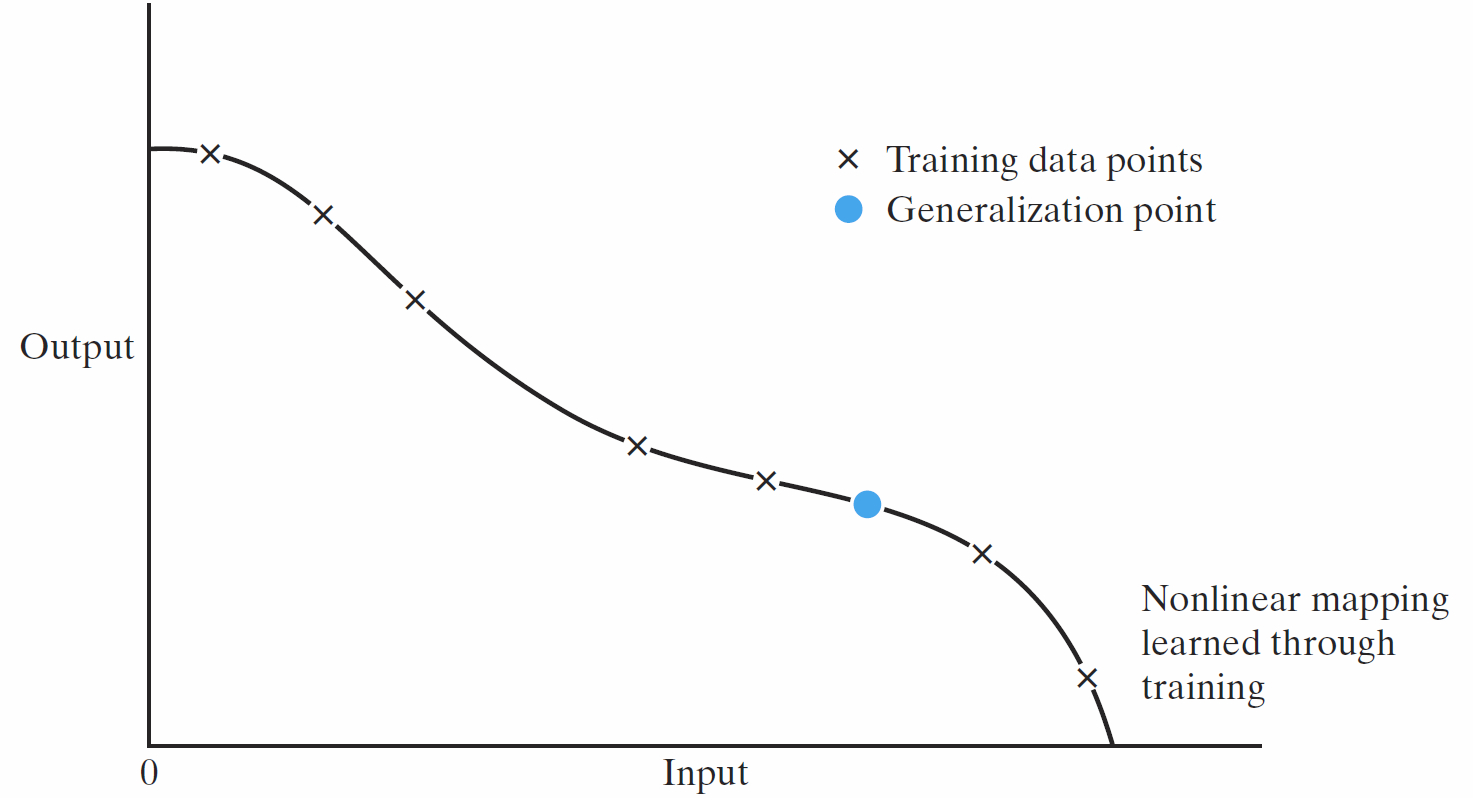
\includegraphics[width=.47\columnwidth]{images/106goodfitting}
	  \label{fig:106goodfitting}  }
  \quad
 % \hfill
  \subfloat[Bad fitting.]{
	  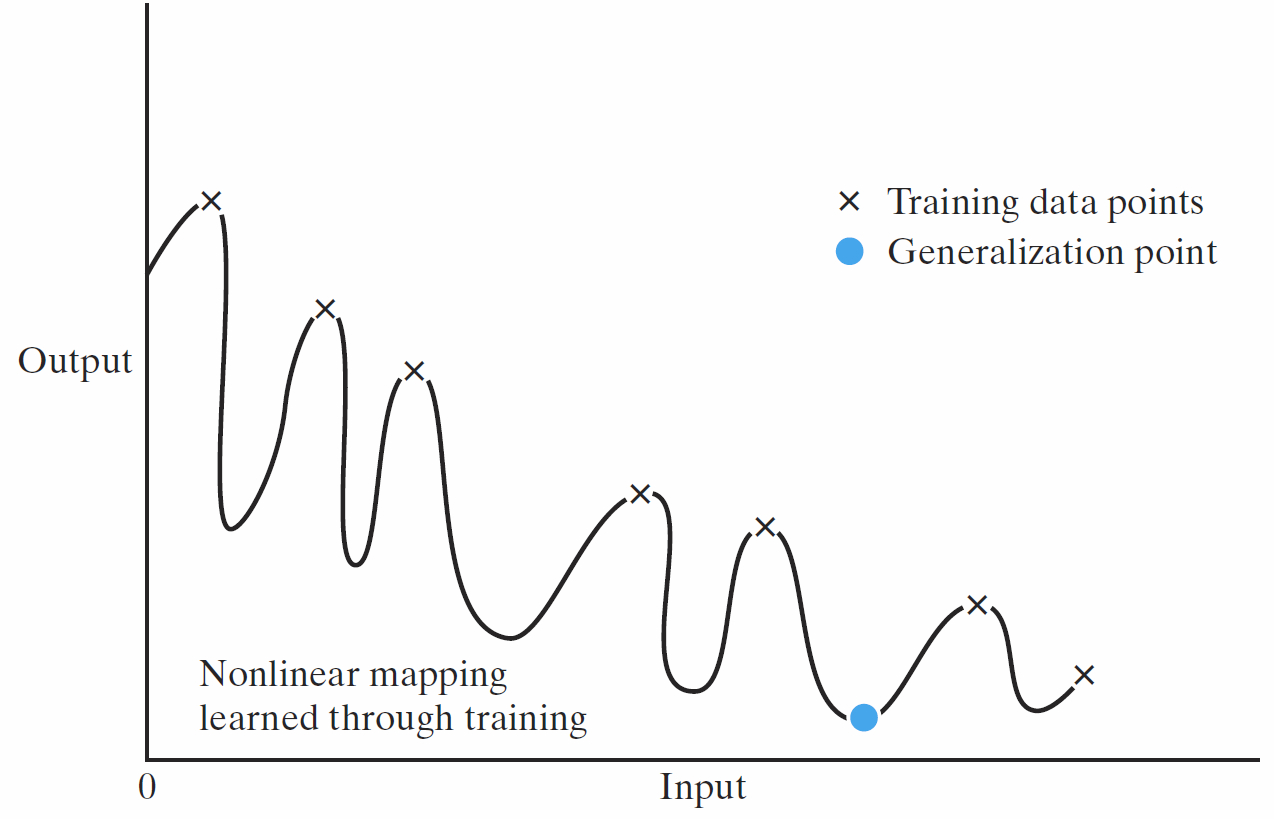
\includegraphics[width=.47\columnwidth]{images/107badfitting}
	  \label{fig:107badfitting}
  }
 % \hfill\null
  \caption[Fitting.]{Fitting, or agreement, between data point and
  regression, or interpolation, functions
  \cite{RefWorks:158}.}
  \label{fig:108fitting}
\end{figure}

Correctly computed input-output mapping is a synonym of a well $generalized$
network, and of good nonlinear interpolation of the inputs, as in Fig. 
\ref{fig:106goodfitting}. On the other hand, an excessive amount of
training samples, known as $overfitting$, leads to poor generalization, see 
Fig. \ref{fig:107badfitting}. Also the architecture of the neural network and
physical complexity of the problem influence the generalization.
A good rule of thumb requires the size of the training sample to be of the same
order of magnitude of the ratio between (a) the total number of free parameters 
(i.e., synaptic weights and biases) in the
network and (b) the fraction of classification errors permitted on test
data (e.g., the mean square value of the estimation error).

\section{Cross validation}
\label{sec:crossvalidation}

A computationally efficient training and the evaluation of good generalization
can be performed with the statistical tool of \textit{cross-validation}.
The available data are randomly divided in the following subsets:

\begin{enumerate}
  \item{training samples subset,}
  \item{generalization (or validation, or early stopping) samples subset,}
  \item{test samples subset.}
\end{enumerate}

For instance, every ten epochs the training is halted and the validation error
(or the cost function) is evaluated with the partially trained network over the
validation set.
Then the training is resumed.
This continues until the learning curve of the error for the validation set
reaches a local minimum, a condition that should happen sooner (i.e., in a
minor number of loops) than the falling of the learning curve for the training
set (cost function \acs{EAVN}) under the prescribed limit.
At this point the output of the trained network is evaluated over the test
subset to evaluate its generalization performances.

\section{ANNs training for DEM identification}
\label{sec:annstrainingfordemidentification}

Following the best practice suggested by Vaferi et al. \cite{RefWorks:150}, we
used $MLPNN$.
Further, the quality of the \acs{ANN} data had to be examined critically. 
Haykin \cite{RefWorks:158} 
suggested considering the quality of (a) \acs{ANN} training process and (b) the
subsequent data generation based on the inputs provided.
Task (a) is particularly important
when dealing with experimental training data, and
usually addressed
by noise-corrupted pattern calibration
and by comparison with standard statistical methods.
However, our training pool was numerical and extensive, 
and the particles in our simulations were inserted using a random
seed value.
For vast amounts of training data, the effect of noise-corrupted patterns is
negligible, see Haykin \cite{RefWorks:158}.
Thus, in our work task (b) was more challenging.
Once trained, the \acs{ANN} were fed
combinations of \acs{DEM} parameters. 
We tried different methods to generate these combinations. 
Our first attempt consisted of assigning parameters to the investigated
variables in even increments from the minimum to the maximum values. 
For example, the \acs{CoR} ranged from 0.5 to 0.9, and thus the first value was
0.5, the second 0.508163, and so on.
To increase generalization, we decided to follow a different approach: 
random value generators created the number of required values in the defined
ranges for each parameter investigated.
These were combined and used as input.\\
